%This is the first real chapter of this thesis. Other chapters can be easily referenced, for example the introduction can be found as Chapter \ref{chapter:introduction}. Sections and/or subsections need to be labeled before one can reference them. See Section \ref{sec:second-section} for an example.

%\section{First Section of the First Chapter}
%Some text in the first section.
%\subsection{First Subsection}
%As well as some text in this subsection.
%\subsubsection{First Subsubsection}
%The Table of Contents only goes 3 layers deep (Chapter - Section - Subsection) so this subsubsection is not seen there.

%\section{Second Section of the First Chapter}\label{sec:second-section}

Projektis kasutatud spordikell on Polar RC3 GPS.
Konkreetne mudel on toodetud aastal 2013, kella tähtsamad omadused on integreeritud GPS moodul, mis suudab arvet pidada alguspunkti üle ning kasutajat sinna tagasi suunata, täpselt kiirust ja distantsi mõõta ning ühilduvus mitmete lisasensoritega, millega saab mõõta südametööd, rattasõidu andmeid ja muud.

\section{Kella riistvara}\label{sec:riistvara}
\begin{figure}[ht]
    \centering
    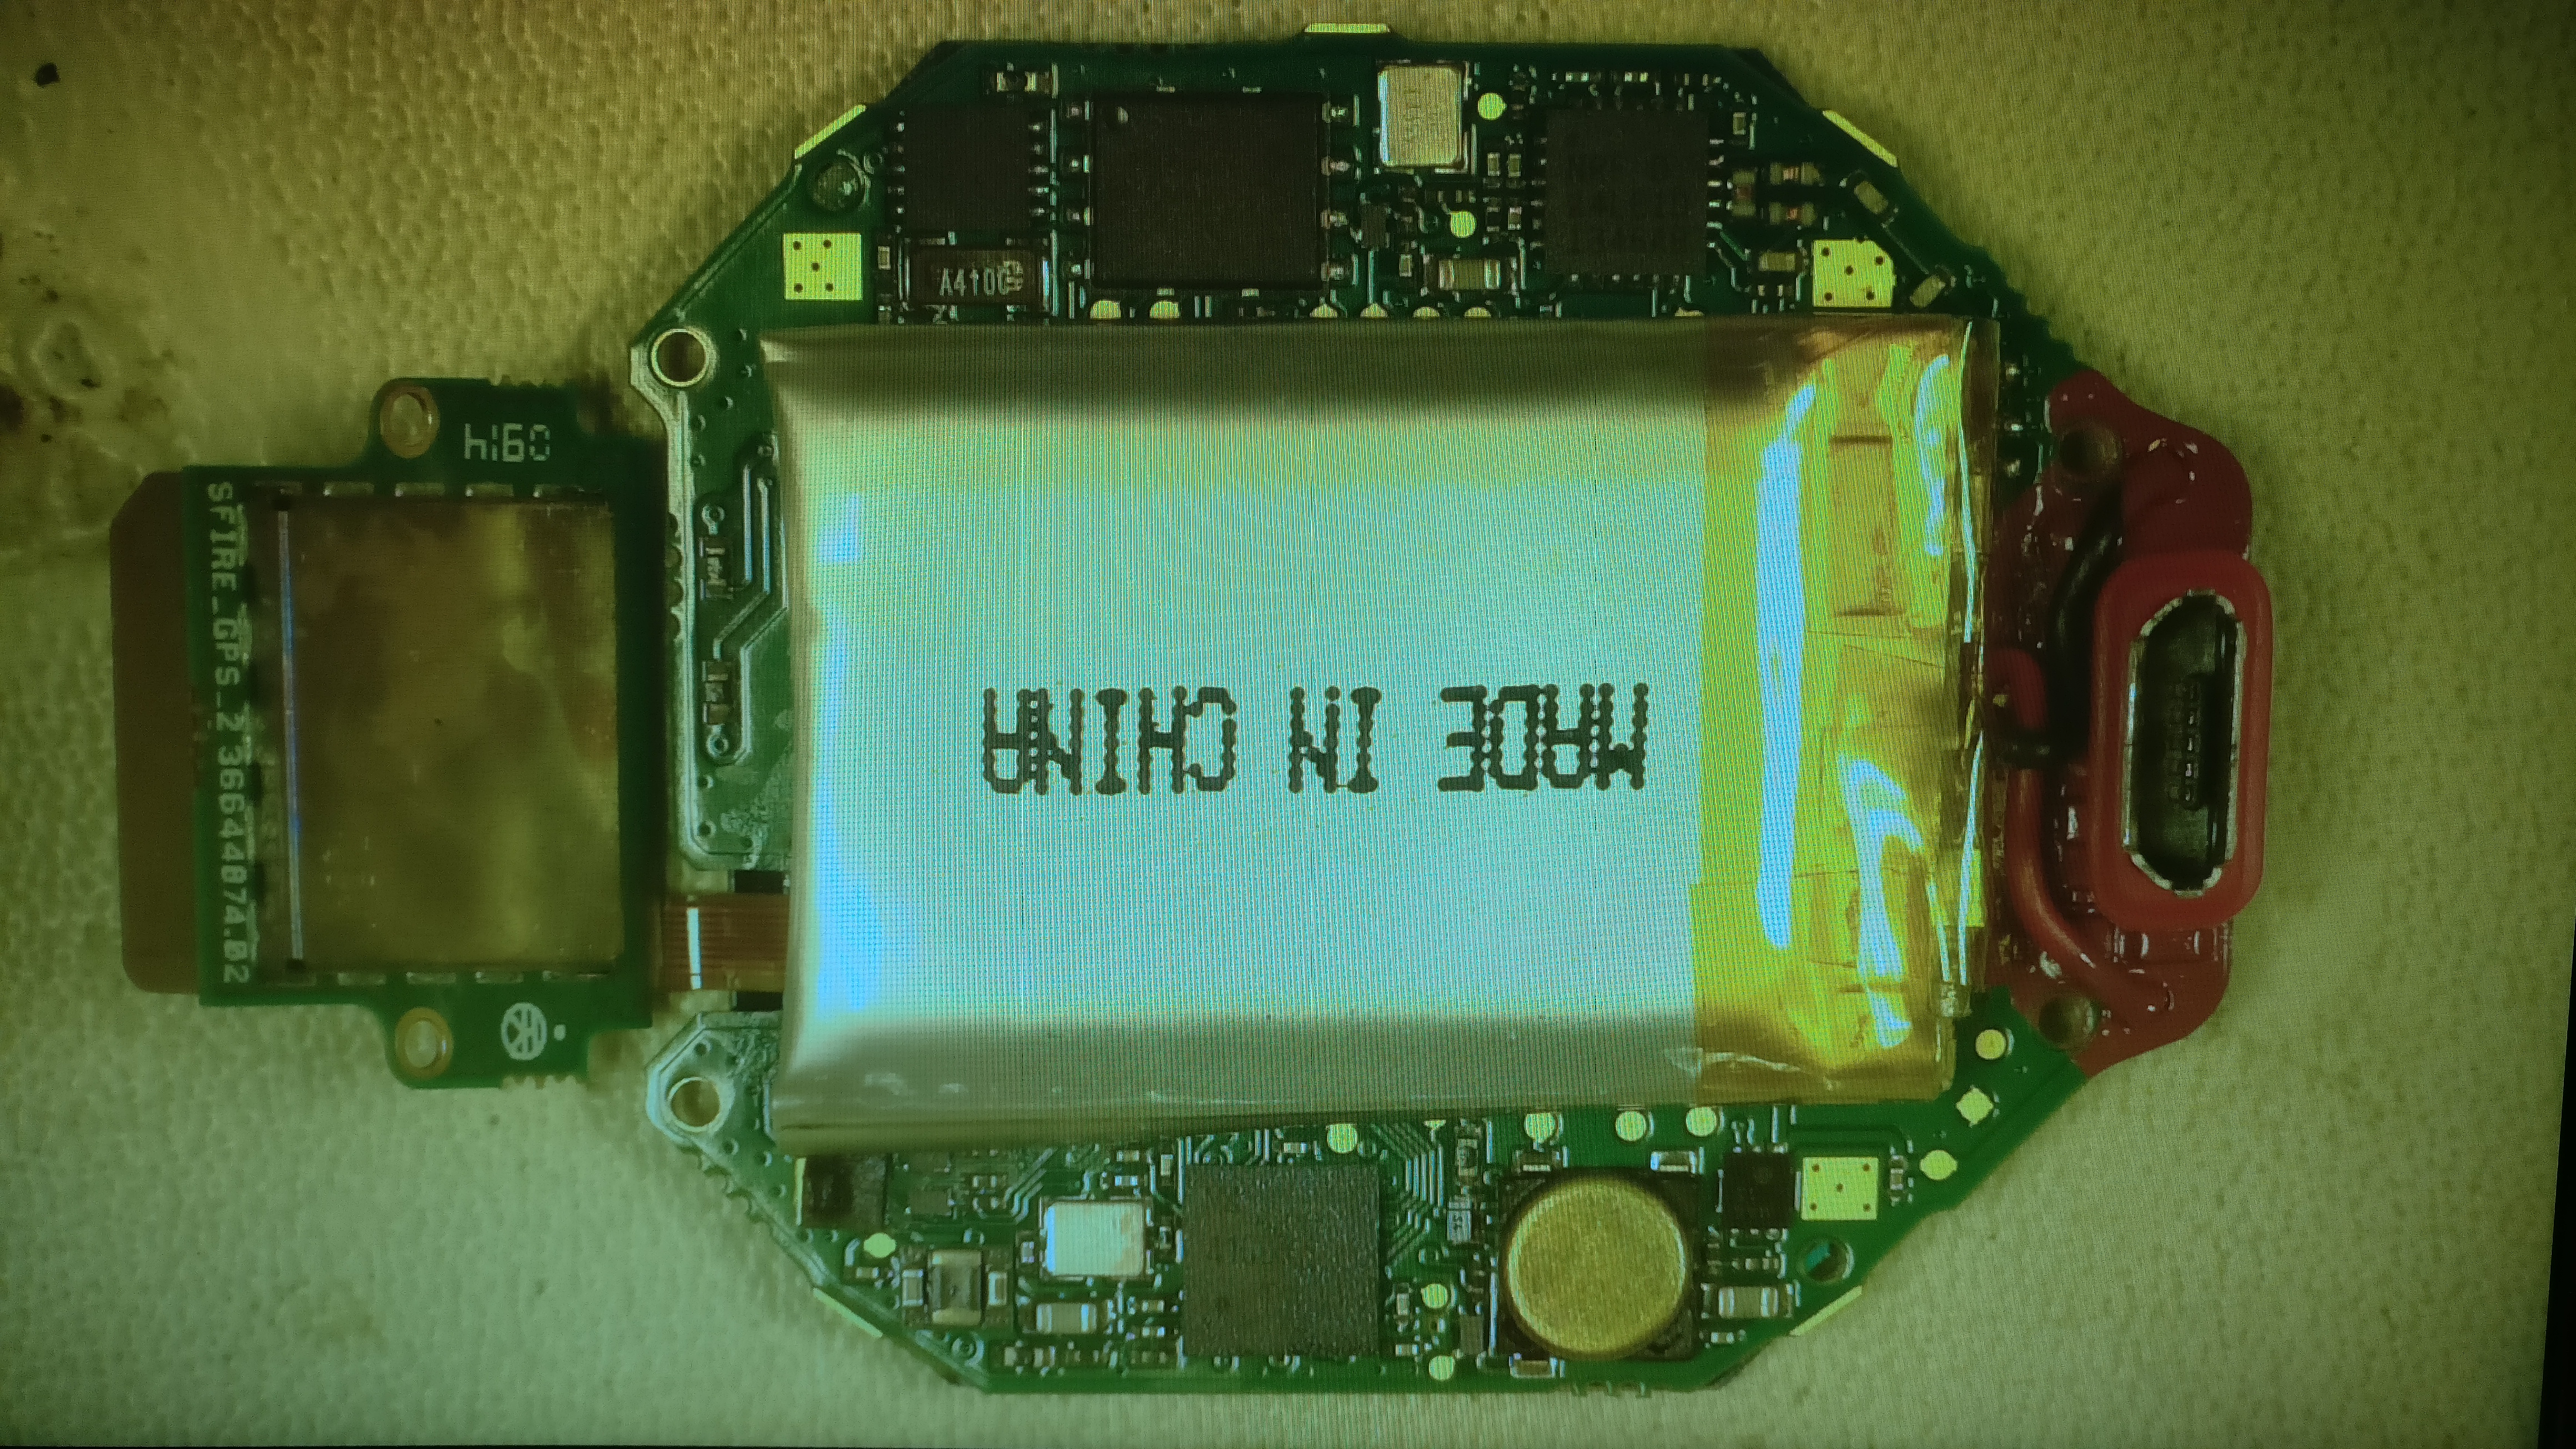
\includegraphics[width=.5\textwidth]{figures/watch.jpg}
    \caption{\textit{Pilt kella sisemusest}}
    \label{fig:watch}
\end{figure}

Projekti alguses tutvuti ka kella riistvaraga, võttes kell lahti ja uurides selle komponente ning otsides andmeliine, mida oleks lihtne füüsiliselt jälgida, et saada paremini aimu kella töötamisest.
Kuna kella pidi saama ka hiljem kasutada, ei hakatud antud projekti käigus eemaldama kella komponente emaplaadilt, et neid lähemalt uurida.
Kella riistvara kohta avalikku dokumentatsiooni ei leitud ning kella enda emaplaati uurides ka ei olnud lihtne aru saada, millised konkreetsed detailid sellel kasutatud olid.
Kella uuriti mikroskoobi all ning iga komponendi kohta pandi kirja kõik informatsioon, mis oli võimalik leida.
Hiljem internetist nende komponentide kohta informatsiooni otsimine ei andnud tulemusi, kuna ei olnud võimalik piisavalt täpselt otsida.

